\documentclass[11pt,a4paper,landscape]{article}
\usepackage[utf8]{inputenc}
\usepackage[english]{babel}
\usepackage{multicol}
\usepackage[margin=0.5in]{geometry}
\usepackage{amsmath}
\usepackage{amssymb} 
\usepackage{enumerate}
\usepackage{fancyhdr}
\usepackage{graphicx}
\usepackage{wrapfig}

\graphicspath{ {./images/} }

\everymath{\displaystyle}
\pagestyle{fancy}
\fancyhf{}

\renewcommand{\headrulewidth}{0pt}
\renewcommand{\footrulewidth}{2pt}

\lfoot{\bfseries Prashant Dhirendra : prashant.dhiru@gmail.com} 
\begin{document}
\begin{multicols*}{3}


\begin{tabbing}
{\bfseries {\Large Cartesian System}}\\
{\bfseries  point co-ordinate:} \\
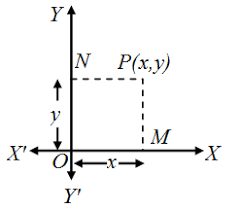
\includegraphics[scale=0.4]{point}\\

{\bfseries  Note:} if both the axis are not ${\bot}^{ar}$,\\ then they are called {\bfseries  oblique axes}\\\\
{\bfseries  Polar co-ordinate:} \\
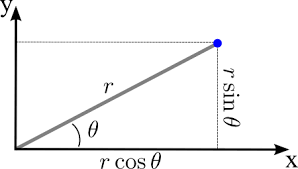
\includegraphics [scale=0.4]{cordinate}\\
$ x= rcos\theta$ \hspace{15mm} \= $y=rsin\theta$\\
$r=\sqrt{x^2+y^2}$ \> $\theta=\tan^{-1} \left ( \frac{x}{y} \right )$\\ \\
{\bfseries  Distance b/w 2 points } $P(x_1,y_2) \quad Q(x_2,y_2)$\\
$PQ = \sqrt{{(x_2-x_1)}^2 + {(y_2-y_1)}^2}$\\ \\
distance from origin : \=$\sqrt{x^2 + y^2}$\\ \\
polar distance : $\sqrt{r_1^2 + r_2^2 - 2 r_1 r_2 \cos (\theta_1 - \theta_2)}$
\end{tabbing}
{\bfseries{\Large Application of Cartesian System}}\\ \\
{\bfseries  For 3 points ABC:} \\
find AB, BC and CA, then if following :
\begin{tabbing}
sum of any two equal to third \hspace{10mm} \= collinear\\
$AB = BC = CA$ \> equilateral $\triangle$\\
any two equal \> isosceles $\triangle$\\
$AB^2 + BC^2 = CA^2$ \> right angle $\triangle$\\

{\bfseries  For 4 points A,B,C and D :} \\
find AB, BC, CD and DA then if following :\\
$\qquad $\underline{$AB = BC = CD = DA$} \\
$\qquad \qquad  AC = BD$ \hspace{20mm} \= square\\
$\qquad \qquad AC \neq BD$ \> rhombus\\

$\qquad $\underline{$AB = CD$ and $BD = DA$} \\
$\qquad \qquad  AC = BD$ \> rectangle\\
$\qquad \qquad AC \neq BD$ \> parallelogram\\
\end{tabbing}
{\bfseries{\Large Application of Cartesian System}}\\ \\
\begin{tabbing}
internal division \hspace{3mm} \=$\left ( \frac{m_1 x_2 + m_2 x_1}{m_1+ m_2}, \frac{m_1 y_2 + m_2 y_1}{m_1+ m_2} \right )$\\ \\
external division \> $\left ( \frac{m_1 x_2 - m_2 x_1}{m_1- m_2}, \frac{m_1 y_2 - m_2 y_1}{m_1- m_2} \right )$\\ \\
mid point \> $\left ( \frac{ x_1+ x_2}{2}, \frac{y_1 +  y_2}{2} \right )$\\ \\
division by line : the line $ax+by+c=0$ divides the\\ line PQ in the ratio \> $\quad \frac{-ax_1+by_1+c}{ax_2+by_2+c}$ \\ \\
co-ordinates of any point on the line segment joining\\ two pointts are \>$\left ( \frac{ x_1+ \lambda x_2}{1+\lambda}, \frac{y_1 +  \lambda y_2}{1+\lambda} \right )$\\ \\
Division by axes\\
$\qquad \qquad$ x-axis \>  y-axis\\\\
$\qquad \qquad\frac{-y_1}{y_2}$ \> $\frac{-x_1}{x_2}$\\ \\
\end{tabbing}
\vfill\null
\columnbreak
%
%
%
{\bfseries{\Large Area of Triangle}}\\ \\
$
\triangle ABC = \frac{1}{2}
\begin{vmatrix}
x_1 & y_1 & 1\\
x_2 & y_2 & 1\\
x_3 & y_3 & 1\\
\end{vmatrix}\\ \\
$
collinear \hspace{10mm}$\Rightarrow Area = 0$\\
Area by co-ordinate axes and line is $\frac{c^2}{2ab}$
for Equilateral $\triangle$ \\
$area = \frac{\sqrt3}{4}side^2 = \frac{1}{\sqrt3}height^2$\\ \\
%
%
%
{\bfseries{\Large Area of Quadrilateral}}\\ \\
$
\triangle ABC = \frac{1}{2}
\begin{vmatrix}
x_1 & y_1 & 1\\
x_2 & y_2 & 1\\
x_3 & y_3 & 1\\
x_4 & y_4 & 1\\
\end{vmatrix}\\ \\
$
collinear \hspace{10mm}$\Rightarrow Area = 0$\\
{\bfseries Two opp. vertices $(x_1,y_1)$ and $(x_2,y_2)$ of rectangle are given}\\
$$
area = 
\begin{vmatrix}
(y_2 - y_1) & (x_2 - x_1)
\end{vmatrix}
$$
%
%
%
{\bfseries{\Large Area of Triangle using Polar}}\\ \\
$
\begin{aligned}
\qquad \qquad \triangle = \frac{1}{2}
\{
	&r_1 r_2 \sin(\theta_2 -\theta_1)+\\
	&r_2 r_3 \sin(\theta_3 -\theta_2)+\\
	&r_3 r_1 \sin(\theta_1 -\theta_3)
\}
\end{aligned}$\\
%
%
%
{\bfseries{\Large Area of Triangle with equation of sides}}\\ \\
if $a_r x +b_r y + c_r = 0$ is given for $r = \{1,2,3\}$\\ \\
$
\triangle = \frac{1}{2C_1 C_2 C_2}
\begin{vmatrix}
a_1 & b_1 & c_1\\
a_2 & b_2 & c_2\\
a_3 & b_3 & c_3\\
\end{vmatrix}
$\\ \\
where $C_1 C_2 and C_3$ are co-factors of $c_1 c_2 and c_3$
\end{multicols*}
\pagebreak
%
%
%
%
%
%
\begin{multicols*}{3}
{\bfseries \noindent {\Large Locus}}\\
if A and B are fixed, then the LOCUS P is
\begin{tabbing}
Circle \hspace{20mm}\=, if $\angle ABC $ = constant \\
Diameter $= AB$ \>,if $\angle ABC = \frac{\pi}{2}$ \\
Ellipse \>,if $PA + PB =$ constant\\
Hyperbola \> if $PA - PB = $ constant\\
\end{tabbing}
%
%
%
{\bfseries \noindent {\Large Different Form of Eq of St. Line}}
\begin{tabbing}
{\bfseries {General Equation }}\hspace{5mm} \= $Ax+By+C=0$\\ \\
{\bfseries {Slope Intercet form }}\hspace{5mm} \> $y = mx+c$\\
\> m = slope , c= y intercept \\ \\
{\bfseries {Point Slope form }}\> $(y-y_1)= m(x-x_1)$\\ \\
{\bfseries {Two Point form }}\> $(y-y_1)= \frac{(y_2-y_1)}{x_2-x_1}(x-x_1)$\\ \\
{\bfseries {Intercept form }}\> $\frac{x}{a}+\frac{y}{b}=1$\\ \\
{\bfseries {Normal or $\bot^{ar}$ form }}\> $x\cos\alpha + y\sin\alpha = p$\\ \\
{\bfseries {Parametric form }}\> $\frac{x-x_1}{\cos\theta} = \frac{y-y_1}{\sin\theta}= r$\\
\end{tabbing}
%
%
%
{\bfseries \noindent {\Large Position of a Point Relative to a Line}}\\
\begin{itemize}
	\item $P(x_1,y_1) , Q(x_2,,y_2)$ are on \underline{same side of line} $ax+bx+c=0$, if $ax_1+by_1+c$ and $ax_2+by+c$ have same sign or vice versa
	\item $(x_1,y_1)$ is on the origin side of the line$ax+bx+c=0$, if $ax_1+by_1+c$ and$c$ have same sign or vice versa 
\end{itemize}
\vfill\null
\columnbreak
%
%
%
{\bfseries \noindent {\Large Angle Between Two Lines}}\\
{\bfseries {when slope is given }}
$$\tan\theta = \frac{m_1-m_2}{1+m_1m_2}$$
$\parallel \Rightarrow m_1 = m_2 \qquad \bot^{ar}  \Rightarrow m_1 m_2 = -1 $\\
%
$\rule{\linewidth}{1pt}$\\
%
{\bfseries {when eq. of line is given }}\\
suppose $a_1x+b_1y+c_1=0$ and $a_2 x+b_2 y+ c_2=0$ are given
\begin{itemize}
	\item angle :  $ \tan\theta = \frac{a_2 b_1 - a_1 b_2}{a_1 a_2+b_1 b_2}$\\
	\item if lines are $\parallel, \quad \Rightarrow \frac{a_1}{a_2} = \frac{b_1}{b_2}$
	\item if lines are $\bot^{ar}, \quad \Rightarrow a_1 a_2 + b_1 b_2 = 0$
	\item if lines coincides $\quad \Rightarrow \frac{a_1}{a_2}=\frac{b_1}{b_2}=\frac{c_1}{c_2}$
\end{itemize}
%
%
%
{\bfseries \noindent {\Large Equation of a Line Making Angle with Another Line}}\\
the eq of a line passing through P$(x_1,y_1)$ and making an angle $\alpha$ with the line $y= mx+c$\\
$$
y-y_1 = \frac{m\mp \tan\alpha}{1\pm m\tan\alpha}(x-x_1)
$$
{\bfseries \noindent {\Large Concurrency of 3 lines}}\\
all the 3 line meet at a point of intersection 
$$
	\begin{vmatrix}
	a_1 & b_1 & c_1\\
	a_2 & b_2 & c_2\\
	a_3 & b_3 & c_3\\
	\end{vmatrix}
	= 0
$$
%
%
%
{\bfseries \noindent {\Large Distance Between Two $\parallel$ lines}}\\
$$
	d = \frac{| c_1 - c_2|}{\sqrt{a^2 + b^2}}
$$
\vfill\null
\columnbreak
%
%
%
{\bfseries \noindent {\Large Line Passing Through Intersection of Two Lines}}\\
$L_1 \equiv a_1 x+b_1 y+c_1 \qquad  L_2 \equiv a_2 x+b_2 y+c_2 $
$$ \textrm{Line} \Rightarrow L1 + \lambda L2 = 0$$
%
%
%
{\bfseries \noindent {\Large Area of Quadrilateral and Parallelogram}}\\
{\bfseries { Area of Quadrilateral }}  = $ 4 \frac{c^2}{2ab}$\\ \\
{\bfseries { Area of parallelogram }}  = $ \left | \frac{(c_1 - c_2)(d_1 - d_2)}{m_1-m_2} \right |$\\ \\
$y=m_1 x+c_1, y=m_1 x+c_2,y=m_2 x+d_1$ and $y=m_2 x+d_2$ are the eq of sides $\parallel^{gram}$\\ \\
%
%
%
{\bfseries \noindent {\Large Transformation of Axes}}\\
\begin{wrapfigure}{l}{0.4\linewidth}
\centering
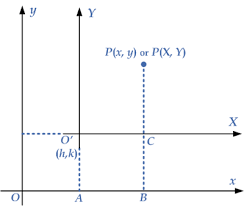
\includegraphics [scale=0.4]{parallel_trans}\\
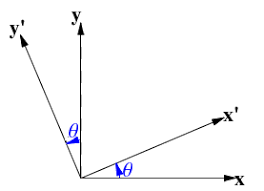
\includegraphics [scale=0.4]{rotational_trans}\\
\end{wrapfigure}
%
{\bfseries { Parallel transformation }}\\
then the co-ordinates of point P with respect to new axis O` will be $$(x-h,y-k)$$
\\ 
%
{\bfseries { Rotational transformation }}\\\\
\begin{tabular}{|| c || c | c|| }
\hline 
 New/Old & x$\downarrow$ & y$\downarrow$ \\[0.5ex]
\hline \hline
 $x'\rightarrow$ & $\cos\theta  $ & $\sin\theta$\\  
 $y'\rightarrow$ & $-\sin\theta  $ & $\cos\theta$\\
\hline
\end{tabular}
\end{multicols*}
\pagebreak
%
%
%
%
%
\begin{multicols*}{3}
{\bfseries \noindent {\Large General Eq of Second Degree}}\\
General Eq. of second degree in x and y is\\
$ax^2+2hxy+by^2+2gx+2fy+c=0$\\ \\
it represents a straight line, if\\
$$
	\Delta = 
	\begin{vmatrix}
		a & h & g\\
		h & b & f\\
		g & f & c\\
	\end{vmatrix}
	=0
$$
$
\textrm{or,} \quad abc+2fgh-af^2 -bg^2 - ch^2 = 0
$\\ \\
%
%
%

{\bfseries \noindent {\Large Eq of Lines Joining the Intersection Points of a Line and Curves to the Origin}}\\
Let $lx+my+n =0$ be the line \\
and $ax^2 + 2hxy+by^2+2gx+2fy+c=0$ be $2^{nd}$ degree curve
\begin{multline*}
ax^2+2hxy+by^2+2gx\left(\frac{lx+my}{-n}\right) \\
+2fy\left(\frac{lx+my}{-n}\right)+c\left({\frac{lx+my}{-n}}\right)^2 =0
\end{multline*}
$\rule{0.45\linewidth}{2pt} \times \rule{0.45\linewidth}{2pt}$\\

\end{multicols*}
\end{document}
